\documentclass[11pt]{article}

\usepackage{amsmath,amsfonts}
\usepackage{graphicx}
\usepackage{microtype}
\usepackage{lmodern}  
\usepackage[T1]{fontenc}

\usepackage[hidelinks]{hyperref}
\usepackage{hyperref}
\usepackage{booktabs}
\usepackage{tikz}
\usepackage[hidelinks]{hyperref}
\usetikzlibrary{positioning, arrows.meta, calc}

\title{Cognitive Amplification vs Cognitive Delegation in Human--AI Systems:
A Metric Framework}

\author{
Eduardo Di Santi\\[4pt]
%University of Colorado Boulder\\[2pt]
%\texttt{eduardo.disanti@colorado.edu}
}
\date{\today}

\begin{document}

\maketitle

\begin{abstract}
Artificial intelligence is increasingly embedded in human decision-making,
where it can either enhance human reasoning or induce excessive cognitive
dependence. This paper introduces a conceptual and mathematical framework
for distinguishing \emph{cognitive amplification}, in which AI improves
hybrid human--AI performance while preserving human expertise, from
\emph{cognitive delegation}, in which reasoning is progressively outsourced
to AI systems.

To characterize these regimes, we define a set of operational metrics:
the Cognitive Amplification Index ($CAI^*$), the Dependency Ratio ($D$),
the Human Reliance Index ($HRI$), and the Human Cognitive Drift Rate ($HCDR$).
Together, these quantities provide a low-dimensional metric space for
evaluating not only whether human--AI systems achieve genuine synergistic
performance, but also whether such performance is cognitively sustainable
for the human component over time.

The framework highlights a central design tension in human--AI systems:
maximizing short-term hybrid capability does not necessarily preserve
long-term human cognitive competence. We therefore argue that human--AI
systems should be designed under a \emph{cognitive sustainability}
constraint, such that gains in hybrid performance do not come at the cost
of degradation in human expertise.
\end{abstract}

\section{Introduction}

Artificial intelligence (AI) systems are increasingly embedded in
human decision-making across domains such as engineering, medicine,
finance, and scientific work. In these settings, AI is often introduced
with the promise of improving task performance, increasing efficiency,
and supporting better decisions. Within human-centred AI, however,
the quality of a system cannot be assessed solely in terms of immediate
performance gains; it must also be evaluated in terms of how it shapes
human oversight, agency, and competence over time.

This issue has become increasingly important in human--AI interaction
research. Although AI systems can improve human performance in some
tasks, empirical work shows that human--AI combinations do not
consistently outperform the best standalone agent, especially in
decision-making settings. In parallel, research on automation bias,
overreliance, and cognitive offloading suggests that AI assistance may
improve short-term outcomes while reducing independent verification,
critical scrutiny, and unaided task performance.

These findings point to a fundamental evaluation gap. Existing
human--AI assessment practices tend to emphasize hybrid task performance,
but offer limited support for distinguishing between two importantly
different interaction regimes. In one regime, AI acts as a cognitive
amplifier: it improves hybrid performance while preserving or even
strengthening the human's ability to reason independently. In the
other, AI functions as a source of cognitive delegation: reasoning is
progressively outsourced to the system, increasing dependency and
creating the risk that human competence deteriorates over time.

This paper proposes a conceptual and mathematical framework for
analyzing this distinction. We introduce four operational quantities:
the Cognitive Amplification Index ($CAI^*$), the Dependency Ratio ($D$),
the Human Reliance Index ($HRI$), and the Human Cognitive Drift Rate
($HCDR$). Together, these metrics are intended to support the evaluation
of human--AI systems not only in terms of system-level gains, but also
in terms of whether those gains are cognitively sustainable for the
human component.

The main contribution of the paper is therefore threefold.
First, we distinguish cognitive amplification from cognitive delegation
as two qualitatively different regimes of human--AI interaction.
Second, we propose a compact metric framework for characterizing hybrid
performance, AI dominance, and the evolution of unaided human capability.
Third, we derive design implications for human--AI systems that aim to
improve performance without eroding long-term human expertise.

The contributions of this paper are as follows:

\begin{enumerate}
\item We introduce a conceptual distinction between \emph{cognitive amplification}
and \emph{cognitive delegation} as two qualitatively different regimes of
human--AI interaction.

\item We propose a compact metric framework for characterizing these regimes
through four operational quantities: the Cognitive Amplification Index
($CAI^*$), the Dependency Ratio ($D$), the Human Reliance Index ($HRI$),
and the Human Cognitive Drift Rate ($HCDR$).

\item We show how these metrics distinguish between immediate hybrid
performance gains and the longer-term preservation or erosion of unaided
human competence, thereby making \emph{cognitive sustainability} an explicit
evaluation target for human--AI systems.

\item We derive design implications for human--AI systems, arguing that
interfaces and workflows should be evaluated not only by hybrid task
performance, but also by whether they preserve meaningful human cognitive
engagement over time.
\end{enumerate}



The paper proceeds as follows. Section 2 reviews related work on
human--AI collaboration, automation bias, cognitive offloading, and
human-centred AI. Section 3 introduces the system model and the proposed
metrics. Section 4 discusses how these metrics define qualitatively
different regimes of human--AI collaboration. Section 5 derives design
implications for cognitively sustainable human--AI systems, and
Section 6 discusses limitations and directions for empirical validation.


\section{Related Work}

\subsection{Human--AI collaboration and complementarity}

Recent work on human--AI collaboration emphasizes that the effectiveness
of hybrid systems depends not only on AI capability, but also on the
quality of interaction, task structure, and the extent to which human
and artificial agents contribute complementary information or capabilities.
Research on complementarity in human--AI decision-making argues that
useful collaboration arises when differences in access to information,
representational strengths, or error patterns can be productively combined,
rather than when one agent merely replicates the function of the other.
Related work further shows that hybrid performance should not be assumed:
in many settings, human--AI combinations fail to outperform the best
standalone component, making the design of effective interaction protocols
a central problem rather than a secondary implementation detail.

These findings motivate the need for evaluation frameworks that go beyond
raw hybrid accuracy. If human--AI performance gains are highly contingent
on the organization of the interaction, then the assessment of such systems
should include not only whether performance improves, but also how that
improvement is achieved and whether it depends on preserving an active
human cognitive role.

\subsection{Overreliance, automation bias, and cognitive offloading}

A large body of work has shown that humans often over-rely on automated
decision aids. Research on automation bias describes the tendency of
users to give excessive weight to automated recommendations, reduce
independent verification, and inherit system errors, particularly in
high-stakes or cognitively demanding tasks. More recent literature on
AI overreliance extends these concerns to modern human--AI systems,
showing that the presence of AI assistance can alter judgment strategies,
reduce scrutiny, and create a misleading appearance of robust
human-in-the-loop oversight.

These concerns are closely related to the broader literature on cognitive
offloading. Offloading research shows that external aids can improve
immediate task performance while also changing how users remember,
reason, and allocate mental effort. In the context of AI-assisted
decision-making, this raises an important possibility: a system may
increase short-term hybrid performance while simultaneously weakening
the user's capacity to perform comparable tasks without assistance.
This distinction is central to the present paper.

\subsection{Human-centred AI and cognitively sustainable interaction}

Human-centred AI has increasingly been framed not only as a matter of
usability or explainability, but as a broader design commitment to
maintaining meaningful human agency, oversight, and participation in
AI-supported work. Within this perspective, good human--AI interaction
requires more than accurate model outputs. It also requires interfaces
and workflows that calibrate trust, support critique, expose uncertainty,
and preserve the human's ability to reason about the task.

However, current evaluation practices in human--AI systems still focus
primarily on immediate hybrid performance. Comparatively less attention
has been paid to whether interaction designs preserve human competence
over time. The present work contributes to this gap by proposing a
framework that explicitly distinguishes between performance gains that
reflect cognitive amplification and those that mask progressive cognitive
delegation.

\subsection{Conceptual foundations of human and artificial cognition}

The distinction proposed in this paper is also informed by longer-standing
conceptual debates about the nature of human cognition and artificial
computation. Searle's Chinese Room argument \cite{searle1980} remains a
canonical challenge to the idea that formal symbol manipulation alone
constitutes understanding. This argument is relevant here not because
the present paper attempts to resolve the philosophy of mind, but because
it highlights a basic asymmetry: human and artificial systems may produce
similar outputs while relying on fundamentally different cognitive
processes.

Related philosophical work by Byrne on computation, self-knowledge, and
the transparency of belief formation further motivates the concern that
treating AI as a functional substitute for reasoning may alter the human
subject's relation to its own cognitive processes \cite{byrne-minds-machines,byrne-kim-2012,byrne2018}. In a different but complementary register,
Solms emphasizes the embodied, affective, and homeostatic grounding of
human cognition and consciousness, suggesting that human intelligence is
not exhausted by abstract information processing alone \cite{solms2021,solms-friston-2019}. Taken together, these perspectives reinforce the
motivation for distinguishing between systems that support human
reasoning and systems that progressively displace it.

The present paper does not claim that these philosophical positions
directly entail the proposed metrics. Rather, they provide a conceptual
background for why the preservation of human cognitive competence should
be treated as a first-class concern in the design and evaluation of
human--AI systems.


\section{System Model}

Consider a hybrid system composed of a human and an AI agent.

\begin{equation}
S = H + A
\end{equation}

where $H$ represents the human component and $A$ the artificial
component. This expression is not intended as a literal additive
decomposition of intelligence, but as a compact representation of a
coupled human--AI system whose effective behavior emerges from the
interaction between both components.

Human intelligence, in particular, involves forms of understanding,
judgment, and self-monitoring that are not exhausted by any single
performance measure. Nevertheless, to evaluate whether AI amplifies
or displaces human cognitive function, an operational projection of
capability is required.

We therefore define the effective problem-solving capacity of the
system as

\begin{equation}
Q(S) = Q(H,A)
\end{equation}

where $Q$ denotes an operational measure of task-relevant cognitive
performance within a given domain, not a measure of intelligence in
the abstract.

Human performance alone corresponds to

\begin{equation}
Q_H = Q(H)
\end{equation}

while AI capability alone corresponds to

\begin{equation}
Q_A = Q(A)
\end{equation}

The hybrid system capability is therefore

\begin{equation}
Q_{HA} = Q(S).
\end{equation}

The central question of this paper is not whether AI reproduces human
intelligence in full, but whether AI systems enhance human cognitive
agency or progressively replace its practical exercise.


\section{Cognitive Amplification}

In the ideal case, AI functions as a cognitive amplifier. The hybrid
system exhibits a form of synergy in which machine assistance extends
human problem-solving capacity without suppressing the active exercise
of human judgment.

As a conceptual model, this may be written as

\begin{equation}
Q_{HA} = Q_H + Q_A + \alpha Q_H Q_A
\end{equation}

where $\alpha$ represents the strength of the human--AI interaction.
When $\alpha > 0$, the coupled system exhibits a positive interaction
term beyond the isolated contribution of either component.

This expression should be interpreted as an idealized representation of
human--AI synergy rather than as a literal empirical law. In real
applications, performance measures are often bounded and strongly
task-dependent, and hybrid performance does not generally scale in a
strictly additive fashion. For this reason, the practical analysis
developed in the remainder of the paper relies on relative performance
metrics that compare the hybrid system against the relevant standalone
baselines.

\section{Metrics for Human--AI Collaboration}

The system model introduced above defines three task-level performance
quantities: $Q_H$, $Q_A$, and $Q_{HA}$. The metrics introduced in this
section are derived from these quantities and are intended to
characterize, in a compact and operational way, the regime of
human--AI interaction. They should be interpreted jointly rather than
in isolation: no single metric captures the full picture of whether
a human--AI system is operating in a cognitively sustainable regime.

\subsection{Cognitive Amplification Index}

The Cognitive Amplification Index ($CAI^*$) measures the relative
performance gain of the hybrid system over the best standalone
component:

\begin{equation}
CAI^* = \frac{Q_{HA} - \max(Q_H, Q_A)}{\max(Q_H, Q_A)}.
\end{equation}

This index answers a specific question: does the human--AI combination
outperform both agents working independently? A positive value indicates
genuine synergy; a value of zero means the hybrid merely matches the
best standalone agent; a negative value indicates that the integration
harms overall performance.

\begin{center}
\begin{tabular}{cc}
\toprule
$CAI^*$ & Interpretation \\
\midrule
$> 0$   & Cognitive amplification over best component \\
$= 0$   & Hybrid matches best component (no net gain) \\
$< 0$   & Integration reduces overall performance \\
\bottomrule
\end{tabular}
\end{center}

It is important to note that $CAI^* > 0$ is a necessary but not
sufficient condition for cognitive amplification in the deeper sense
intended by this paper. A system may achieve a positive $CAI^*$ while
simultaneously increasing AI dominance and eroding human competence
over time. The remaining metrics are therefore needed to complete the
picture.

\subsection{Dependency Ratio and Human Reliance Index}

The Dependency Ratio ($D$) measures the degree to which hybrid
performance is anchored to the AI baseline:

\begin{equation}
D = \frac{Q_A}{Q_{HA}}.
\end{equation}

High values of $D$ indicate that the hybrid system performs close to
the AI alone, suggesting that the human contribution is limited and
that the system may be operating in an AI-dominated regime. This is
consistent with empirical work on overreliance and automation bias,
where human operators tend to accept AI recommendations with reduced
independent verification.

The complementary Human Reliance Index ($HRI$) expresses the same
relationship from the perspective of the human contribution:

\begin{equation}
HRI = 1 - D = \frac{Q_{HA} - Q_A}{Q_{HA}}.
\end{equation}

$D$ and $HRI$ do not provide independent information; they are two
perspectives on the same quantity. Together they allow the regime of
human--AI collaboration to be located on a spectrum from
human-dominant to AI-dominated interaction.

\begin{center}
\begin{tabular}{ccc}
\toprule
Range of $D$ & Range of $HRI$ & Qualitative regime \\
\midrule
$< 0.5$      & $> 0.5$        & Human-dominant \\
$0.5$--$0.8$ & $0.2$--$0.5$   & Balanced collaboration \\
$> 0.8$      & $< 0.2$        & AI-dominated, risk of delegation \\
\bottomrule
\end{tabular}
\end{center}

These thresholds are operational heuristics, not universal constants.
Their appropriate values will depend on the domain, task structure,
and acceptable risk profile of the application. In safety-critical
settings, for example, a lower threshold for acceptable $D$ may be
warranted.

\subsection{Human Cognitive Drift Rate}

The first three metrics characterize the state of a human--AI system
at a given point in time. The Human Cognitive Drift Rate ($HCDR$)
addresses a different and arguably more important question: how does
unaided human performance evolve over time as a result of sustained
AI interaction?

Let $Q_H(t)$ denote human task performance measured \emph{without}
AI assistance at time $t$, evaluated through periodic AI-off
assessment blocks in the same task domain. The $HCDR$ is defined as:

\begin{equation}
HCDR = \frac{Q_H(t_2) - Q_H(t_1)}{t_2 - t_1}.
\end{equation}

Two regimes arise naturally:

\begin{itemize}
\item $HCDR \geq 0$: the \textbf{amplification regime}. Unaided human
performance is preserved or improves over time despite sustained AI
assistance. This is more likely when AI scaffolds human reasoning
rather than replacing it directly.

\item $HCDR < 0$: the \textbf{delegation regime}. Unaided human
performance deteriorates over time. This pattern is consistent with
empirical findings on cognitive offloading and automation bias,
where unrestricted AI access can improve immediate assisted performance
while degrading the user's capacity to perform comparable tasks
independently.
\end{itemize}

The $HCDR$ is the metric most directly relevant to the cognitive
sustainability constraint proposed in this paper. A human--AI system
may exhibit positive $CAI^*$ and moderate $D$ while still producing
negative $HCDR$ if the interaction design does not preserve active
human cognitive engagement. Conversely, a system with modest $CAI^*$
but non-negative $HCDR$ may be preferable in domains where long-term
human expertise is a safety or operational requirement.

\subsection{Joint interpretation}

The four metrics introduced above define a compact characterization
space for human--AI systems. Table~\ref{tab:metric_summary} summarizes
their roles and the questions they address.

\begin{table}[ht]
\centering
\begin{tabular}{lll}
\toprule
Metric & Question addressed & Direction of concern \\
\midrule
$CAI^*$ & Does the hybrid outperform the best standalone agent?
        & $CAI^* \leq 0$ \\
$D$     & How dominant is the AI in hybrid performance?
        & $D \to 1$ \\
$HRI$   & How large is the human contribution to hybrid performance?
        & $HRI \to 0$ \\
$HCDR$  & Is unaided human performance preserved over time?
        & $HCDR < 0$ \\
\bottomrule
\end{tabular}
\caption{Summary of proposed metrics and their interpretive roles
in the evaluation of human--AI collaboration regimes.}
\label{tab:metric_summary}
\end{table}

No single metric is sufficient. The most informative characterization
of a human--AI system requires reading $CAI^*$, $D$, and $HCDR$
jointly. In particular, high hybrid performance ($CAI^* > 0$) combined
with high AI dominance ($D \to 1$) and negative drift ($HCDR < 0$)
defines the \emph{automation trap}: a configuration that appears
productive in the short term but is cognitively unsustainable.


\section{Regimes of Human--AI Collaboration}

The metrics introduced above can be interpreted as defining a state space
for human--AI systems. In particular, the pair $(D, CAI^*)$ provides a
useful low-dimensional representation of the interaction regime, where
$CAI^*$ captures the performance gain of the hybrid system over the best
standalone component, and $D$ measures the degree of AI dominance within
the collaboration.

Figure \ref{fig:cognitive_regimes} shows ...

Within this space, qualitatively distinct regimes can be identified.
Human Cognitive Drift ($HCDR$) then determines whether a regime is stable
from the standpoint of long-term human expertise or whether it tends
toward progressive cognitive erosion.

Figure \ref{fig:phase_diagram} shows ...
\begin{figure}[h!]
\centering
\resizebox{0.95\linewidth}{!}{
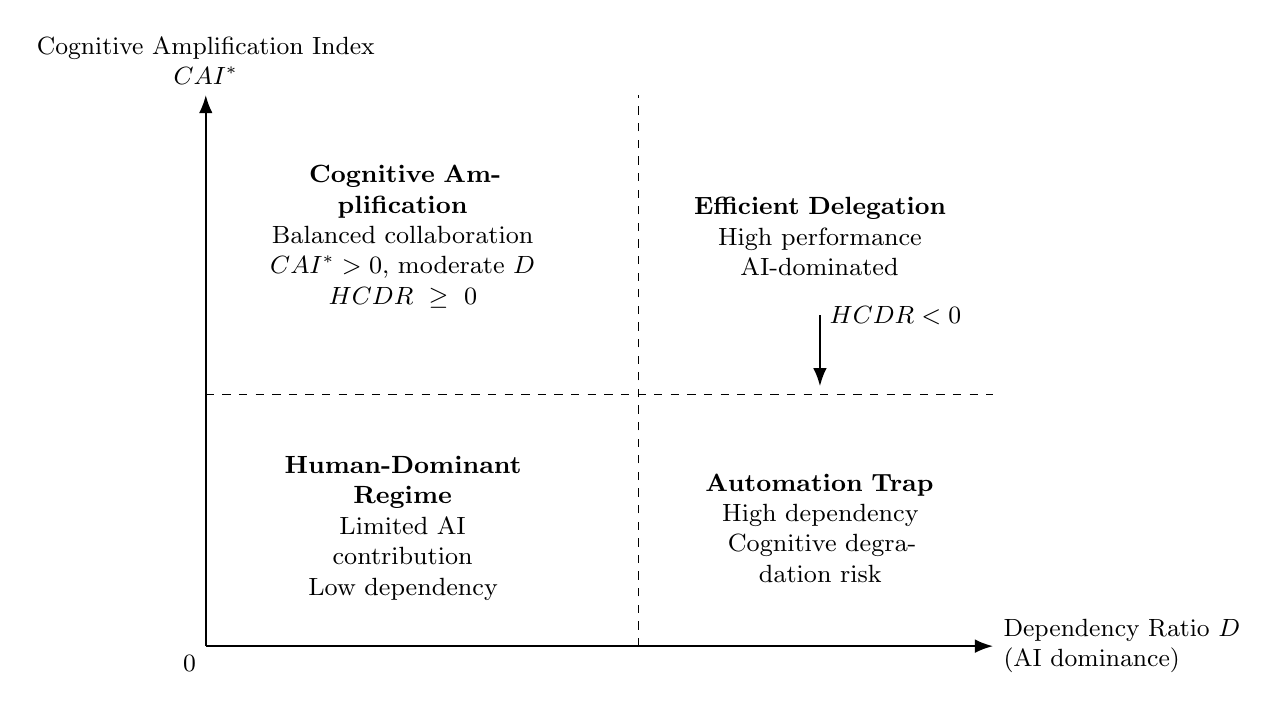
\begin{tikzpicture}[
    >=Latex,
    font=\small
]

% axes
\draw[->, thick] (0,0) -- (10,0)
    node[right, align=left] {Dependency Ratio $D$\\(AI dominance)};
\draw[->, thick] (0,0) -- (0,7)
    node[above, align=center] {Cognitive Amplification Index\\$CAI^*$};

% origin
\node[below left] at (0,0) {0};

% regime boundaries
\draw[dashed] (0,3.2) -- (10,3.2);
\draw[dashed] (5.5,0) -- (5.5,7);

% top-left
\node[align=center, text width=3.4cm] at (2.5,5.2)
{\textbf{Cognitive Amplification}\\
Balanced collaboration\\
$CAI^*>0$, moderate $D$\\
$HCDR\ge0$};

% top-right
\node[align=center, text width=3.2cm] at (7.8,5.2)
{\textbf{Efficient Delegation}\\
High performance\\
AI-dominated};

% bottom-left
\node[align=center, text width=3.2cm] at (2.5,1.5)
{\textbf{Human-Dominant Regime}\\
Limited AI contribution\\
Low dependency};

% bottom-right
\node[align=center, text width=3.2cm] at (7.8,1.5)
{\textbf{Automation Trap}\\
High dependency\\
Cognitive degradation risk};

% HCDR arrow
\draw[->, thick] (7.8,4.2) -- (7.8,3.3);
\node[right] at (7.8,4.2) {$HCDR < 0$};

\end{tikzpicture}
}
\caption{Conceptual phase diagram of human--AI collaboration regimes.
The horizontal axis represents the Dependency Ratio $D$, measuring the
degree of AI dominance in the hybrid system. The vertical axis represents
the Cognitive Amplification Index $CAI^*$, indicating whether the
human--AI system achieves genuine synergy over the best standalone
component. Human Cognitive Drift ($HCDR$) determines whether a regime
preserves or degrades long-term human expertise.}
\label{fig:phase_diagram}
\end{figure}
These regimes illustrate that maximizing hybrid performance $Q_{HA}$
does not necessarily guarantee cognitively sustainable human--AI
collaboration.


\section{Design Implications}

The metric framework introduced above suggests concrete targets
for the design of human--AI systems.
In safety-critical domains, the goal is not only to maximize
short-term hybrid performance, but to maintain
\emph{cognitive amplification} ($CAI^* > 0$),
avoid excessive AI dominance (moderate $D$ and non-trivial $HRI$),
and keep human cognitive drift non-negative ($HCDR \ge 0$).

This leads to three high-level design objectives:

\begin{itemize}
\item sustain positive amplification at the system level
      ($CAI^* > 0$) rather than merely matching the best
      standalone component;
\item avoid AI-dominated regimes in which $D \to 1$ and $HRI \to 0$,
      which are associated with overreliance and automation bias;
\item preserve or improve human-only performance over time
      ($HCDR \ge 0$), preventing cognitive atrophy when AI
      assistance is removed.\cite{cognitive-offloading,designing-ai-expertise}
\end{itemize}

These objectives can be translated into design principles for
interfaces and workflows.
Rather than providing final answers that humans merely accept,
AI systems should scaffold human reasoning and keep users in an
\emph{active} cognitive loop.

Possible design principles include:

\begin{itemize}
\item \textbf{Forcing explanation of reasoning steps.}
      Interfaces can require users to articulate their own
      hypothesis or rationale before revealing AI suggestions
      or detailed explanations.
      This reduces the risk that users simply adopt AI outputs
      without independent analysis and helps maintain
      $HCDR \ge 0$.\cite{cognitive-offloading,ai-pitfalls}
\item \textbf{Exposing uncertainty and model confidence.}
      Communicating calibrated uncertainty, confidence intervals,
      or alternative candidate solutions helps users calibrate
      trust and reduces blind acceptance of AI recommendations.
      This is consistent with recent work on human--AI
      collaborative uncertainty quantification.\cite{human-ai-uq,uncertainty-explainability}
\item \textbf{Requiring human hypothesis generation.}
      Interaction protocols can be structured so that the human
      must generate an initial diagnosis or plan, and the AI
      acts as a critic or augmenter rather than as a primary
      oracle.
      Such designs increase the interpretive visibility of the
      human contribution and make it less likely that
      $D$ approaches one.\cite{designing-ai-expertise,designing-intelligent-organization}
\item \textbf{Supporting exploration rather than final answers.}
      Systems can present evidence, counterfactual scenarios,
      or alternative solution paths that invite exploration,
      instead of single authoritative outputs.
      This shifts the role of AI from answer provider to
      exploration companion, encouraging deeper engagement and
      reducing the risk of long-term skill degradation.\cite{designing-ai-expertise,ai-cognitive-implications}
\item \textbf{Embedding AI-off evaluation blocks.}
      Periodic tasks in which users must operate without AI
      support enable direct measurement of $Q_H(t)$ and thus
      $HCDR$.
      These assessments can be integrated into training,
      simulation, or certification pipelines to detect early
      signs of cognitive delegation.\cite{impact-ai-cognition,cognitive-offloading}
\end{itemize}

From an engineering perspective, these principles suggest that
human--AI systems should be instrumented not only with standard
performance metrics, but also with telemetry that allows continuous
estimation of $CAI^*$, $D$, and $HCDR$.
Such instrumentation would enable organizations to detect when
their human--AI workflows drift from cognitive amplification
toward cognitive delegation, and to redesign interfaces and
training protocols accordingly.\cite{designing-intelligent-organization,automation-bias-ai-act}

\section{Illustrative Measurement of $Q$}

The framework introduced in this paper does not require a universal
measure of intelligence. Instead, $Q$ represents the effective
problem-solving capability of a system within a specific task domain.

In practical settings, $Q$ can be approximated using task-level
performance metrics such as decision accuracy, solution quality,
task completion time, or error rates in controlled problem-solving
environments.

To illustrate this idea, consider a simplified engineering diagnostic
task. An engineer must identify the root cause of a system anomaly
from a set of sensor signals.

Suppose the following performance levels are observed:

\begin{center}
\begin{tabular}{lc}
\toprule
System & Diagnostic Accuracy \\
\midrule
Human alone ($Q_H$) & 0.70 \\
AI alone ($Q_A$) & 0.80 \\
Human + AI ($Q_{HA}$) & 0.92 \\
\bottomrule
\end{tabular}
\end{center}

The Cognitive Amplification Index is then estimated as

\begin{equation}
CAI^* = \frac{Q_{HA} - \max(Q_H, Q_A)}{\max(Q_H, Q_A)}.
\end{equation}

Substituting the observed values:

\begin{equation}
CAI^* = \frac{0.92 - 0.80}{0.80} \approx 0.15.
\end{equation}

The Dependency Ratio becomes

\begin{equation}
D = \frac{Q_A}{Q_{HA}} = \frac{0.80}{0.92} \approx 0.87.
\end{equation}

Its complementary Human Reliance Index is therefore

\begin{equation}
HRI = 1 - D \approx 0.13.
\end{equation}

In this case the hybrid system exhibits a clear gain over the
best individual component ($CAI^* > 0$).
However, the high value of $D$ indicates that hybrid performance
remains strongly anchored to the AI baseline, suggesting an
AI-dominated configuration despite the positive value of $CAI^*$.
This pattern is consistent with empirical findings on overreliance,
where human--AI teams can achieve high immediate performance while
risking long-term degradation of human expertise.\cite{overreliance-ai,humans-inherit-ai-bias}

\subsection{Illustrative Examples of the Framework}

\paragraph{Pharmaceutical Safety Monitoring.}
Consider a pharmacovigilance task in which safety analysts must identify
potential adverse drug reactions from large collections of clinical reports.

Let $Q$ represent the ability to correctly identify safety signals.
Performance can be measured through standard metrics such as recall,
precision, or F1 score.

Suppose the following results are observed in a controlled evaluation:

\begin{center}
\begin{tabular}{lc}
\toprule
System & Signal Detection Recall \\
\midrule
Human experts ($Q_H$) & 0.72 \\
AI model ($Q_A$) & 0.78 \\
Human + AI collaboration ($Q_{HA}$) & 0.91 \\
\bottomrule
\end{tabular}
\end{center}

The resulting Cognitive Amplification Index is

\[
CAI^* = \frac{0.91 - 0.78}{0.78} \approx 0.17.
\]

The Dependency Ratio becomes

\[
D = \frac{0.78}{0.91} \approx 0.86.
\]

The complementary Human Reliance Index is

\[
HRI = 1 - D \approx 0.14.
\]

In this scenario, the hybrid system clearly outperforms both humans
and the AI model alone ($CAI^* > 0$), indicating cognitive amplification
at the system level.
However, the high value of $D$ suggests that hybrid performance remains
close to the AI baseline, placing the team in an AI-dominated regime.
If analysts primarily accept model suggestions without actively
interrogating them, this configuration may drift toward cognitive
delegation, with a risk of long-term degradation of $Q_H(t)$.\cite{impact-ai-cognition,humans-inherit-ai-bias}

\paragraph{Industrial Anomaly Diagnosis.}
Consider an engineering monitoring system in which operators must diagnose
anomalies in a complex industrial process using sensor data.

Let $Q$ represent diagnostic accuracy under time constraints.
Performance can be measured as the proportion of correctly identified
failure modes during simulated operational scenarios.

Assume the following experimental results:

\begin{center}
\begin{tabular}{lc}
\toprule
System & Diagnostic Accuracy \\
\midrule
Human operator ($Q_H$) & 0.68 \\
AI diagnostic system ($Q_A$) & 0.81 \\
Human + AI collaboration ($Q_{HA}$) & 0.95 \\
\bottomrule
\end{tabular}
\end{center}

The Cognitive Amplification Index becomes

\[
CAI^* = \frac{0.95 - 0.81}{0.81} \approx 0.17.
\]

The corresponding Dependency Ratio is

\[
D = \frac{0.81}{0.95} \approx 0.85.
\]

The complementary Human Reliance Index is

\[
HRI = 1 - D \approx 0.15.
\]

If the hybrid interface is designed so that operators must
generate, critique, and refine diagnostic hypotheses---for example,
by requiring explanation of reasoning steps and uncertainty inspection---the
system may sustain a regime of cognitive amplification with
non-negative human cognitive drift.
By contrast, if operators routinely outsource diagnosis to the AI,
empirical findings on automation bias and cognitive offloading suggest
that $Q_H(t)$ may deteriorate, pushing the system into a delegation
regime despite high short-term performance.\cite{automation-bias,cognitive-offloading,impact-ai-cognition}

\section{Discussion}

The framework proposed here does not attempt to measure intelligence
in an absolute sense. Instead, it provides a relative metric system
to evaluate whether AI systems amplify or replace human cognition.

As AI systems become more capable, this distinction becomes critical
for maintaining human intellectual autonomy.

Safety-critical industries such as railway systems, aviation,
pharmaceutical manufacturing, and medical technology depend on
highly trained human expertise for decision making under uncertainty.
In these domains, artificial intelligence should not replace human
judgment but rather amplify the cognitive capabilities of expert
operators. This challenge is closely related to well-documented
phenomena such as automation bias, in which operators may
over-trust automated decision aids and reduce independent
verification \cite{automation-bias,overreliance-ai}.

This observation highlights a fundamental tension in the design of
human--AI systems: maximizing short-term hybrid performance does not
necessarily preserve long-term human expertise. A system that maximizes
$Q_{HA}$ while driving $HCDR < 0$ may achieve short-term efficiency at
the cost of a progressive loss of human expertise.

In this sense, the design of human--AI systems should be guided not
only by immediate hybrid performance, but also by the long-term
\emph{cognitive sustainability} of human expertise. The framework
proposed in this paper provides a way to evaluate whether human--AI
systems operate in a regime of cognitive amplification or cognitive
delegation, and whether such regimes are sustainable over time.

This distinction is particularly relevant in safety-critical
environments, where the degradation of human expertise due to
excessive reliance on automation may introduce systemic risks
\cite{overreliance-ai,automation-bias}.

The present framework therefore suggests that human--AI systems should
be optimized under a sustainability constraint: improvements in hybrid
performance should not come at the expense of negative human cognitive
drift. Formally, this principle can be expressed as

\[
\max Q_{HA}
\quad \text{subject to} \quad
HCDR \ge 0,
\]

which states that gains in hybrid system capability should not be
achieved by degrading the long-term cognitive competence of the
human component.

\section{Conclusion}

Artificial intelligence presents a dual possibility:
it can amplify human intelligence or gradually replace it.

The metric framework proposed in this paper provides a way to
analyze and monitor this transition.
Future work should focus on empirical evaluation
of these metrics in real-world human--AI interaction settings.

In safety-critical domains, the goal of artificial intelligence
should not be the replacement of human cognition but the
amplification of expert judgment.
Systems that increase automation while degrading human expertise
may ultimately reduce, rather than increase, the intelligence of
the overall system.

\bibliographystyle{plain}
\bibliography{references}
\end{document}
